%!TEX root = ../thesis.tex
% ******************************* Thesis Appendix A ****************************

\ifpdf
    \graphicspath{{Appendix1/Figs/Raster/}{Appendix1/Figs/PDF/}{Appendix1/Figs/}}
\else
    \graphicspath{{Appendix1/Figs/Vector/}{Appendix1/Figs/}}
\fi

\chapter{Methods}
\section{Measuring focal length of scan lens}\label{appendix:scanlens}

The focal length of the scan lens was initially unknown but its position for collimation was, and so a reasonable assumption of its focal length was possible.
To compound certainty the focal length was found experimentally.
To accurately measure the focal length of an unknown lens the focal length of a lens of known focal length is needed to collimate the light.
In this experiment the tube lens of focal length \SI{200}{\milli\meter} was used.
By measuring the width of a laser beam prior ($w_{before}$) to and after ($w_{after}$) the collimating lens pair, the magnification is calculated very accurately and the unknown focal length is found by:

\begin{align}
	M=\frac{f_2}{f_1}=\frac{w_{before}}{w_{after}}  \rightarrow \frac{f_2}{M} =f_{1}
\end{align}

To measure a beam width very accurately a straight sharp edge is placed in the beam path and slowly iterated through, the resultant beam power is then measured using a power meter.
To ensure there is no beam cropping on the power meter another lens was used to focus the intensity correctly, the same lens and its position was used in each measurement to keep with consistency.
The beam power was measured and plotted which produces an integrated Gaussian profile (see \eqref{eq:guass_prop}) otherwise known as an error function.
Mathematically this is described by equation~\eqref{eq:knife}.

\begin{align}
	I(x,y) &= I_0 e^{\frac{-2x^2}{w_x^2}}e^{\frac{-2y^2}{w_y^2}}\label{eq:guass_prop}\\\nonumber
	P_{TOT} &= I_0 \int_{\infty}^{\infty}e^{\frac{-2x^2}{w_x^2}} dx \int_{\infty}^{\infty}e^{\frac{-2y^2}{w_y^2}} dy\\\nonumber
	P(X) &= P_{TOT} - \int_{\infty}^{X}e^{\frac{-2x^2}{w_x^2}} dx I_0 \int_{\infty}^{\infty}e^{\frac{-2x^2}{w_x^2}} \\\nonumber
	&= \frac{P_{TOT}}{2} - \sqrt{\frac{\pi}{2}} I_0 \omega_y \int_{\infty}^{X}e^{\frac{-2x^2}{w_x^2}}\\
	& = \frac{P_{TOT}}{2} \left[1 - erf\left(\frac{\sqrt{2}X}{\omega_x}\right) \right] \label{eq:knife}
\end{align}

Fitting of this curve was implemented using MatLAB's curve fitting package which utilises the method of least squares fitting, see Figure \ref{fig:laser_width}.
The fit result produced values of laser beam width as $w_{before} = \SI{3.76\pm0.04}{\milli\meter}$ and $w_{after} = \SI{0.71\pm0.1}{\milli\meter}$.
% The value of $w_{after}$ was supplied in Table \ref{table:laser} however, for posterity is was remeasured locally in case the value had changed or was incorrect.
This gives a magnification $M$ of \SI{5.37 \pm 0.1}{} therefore the focal length of the scan lens is \SI{37.3\pm0.1}{\milli\meter}.
This also showed that the fill of the \SI{12}{\milli\meter} back aperture was \SI{3.76\pm0.04}{\milli\meter} hence the NA of the \num{0.3} objective used would be \SI{\approx 0.094}{}.

\begin{figure}
\centering
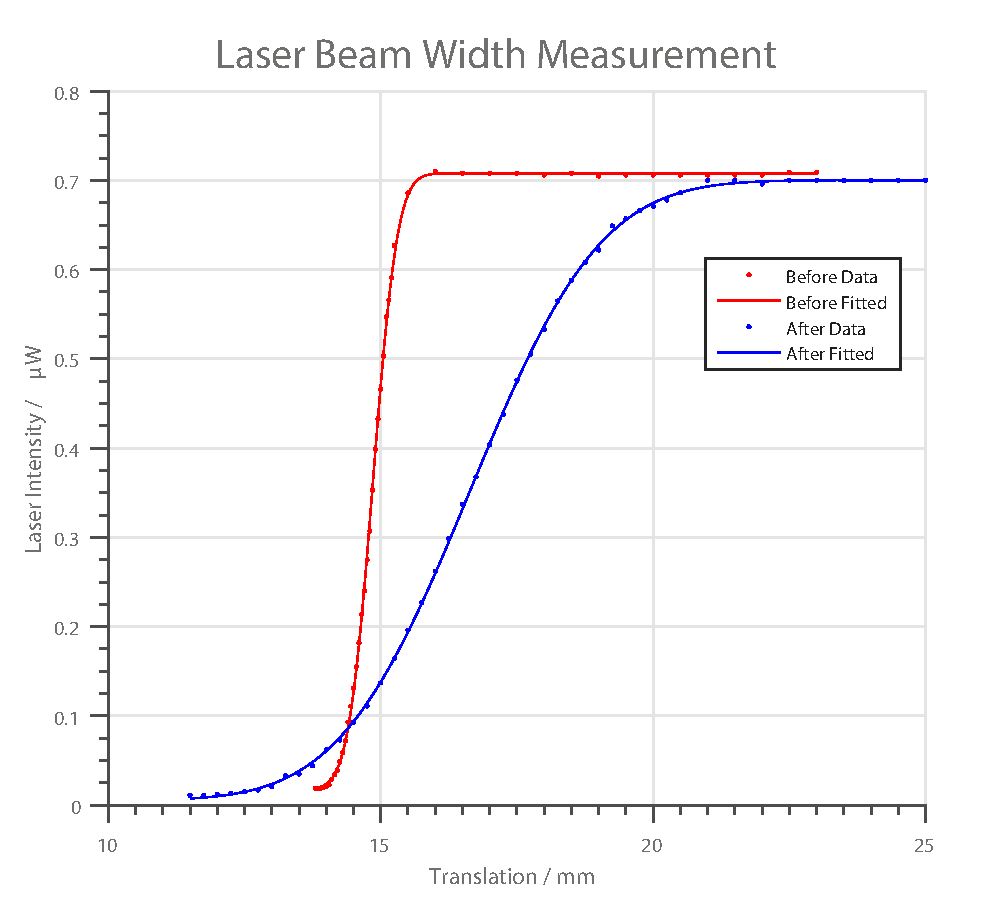
\includegraphics[width=0.7\linewidth]{./laser_width}
\caption[Laser Width Fitting]{Plot showing the fitting of two error functions based on the knife edge translation through a laser beam propagation, producing laser beam widths of $w_{after} = \SI{0.71\pm0.1}{\milli\meter}$ and $w_{before} = \SI{3.76\pm0.04}{\milli\meter}$}
\label{fig:laser_width}
\end{figure}

% \section{System alignments protocol}

%Stationary back apeture.
\chapter{Useful derivations}
\section{Convolution theorem}\label{appendix:convolution_theorem}

Convolution is a mathematical operation between two functions, say $g(t)$ and $f(t)$, with the resultant function being an expression of the overlap of $g$ as it is shifted over $f$ \cite{bracewellFourierAnalysisImaging2004}. Mathematically it can be expressed as an integral over a finite range $\tau$:
\begin{equation}
[f(*g](t) = \int_{-\infty}^{\infty} f(\tau) g(t-\tau)d\tau
\end{equation}

If a Fourier transform is then applied to the convolution of two functions:
\begin{align}
\mathcal{F}([f*g](t)) &= \int_{-\infty}^{\infty} \left[{\int_{-\infty}^{\infty} f(\tau)} g(t-\tau)d\tau\right] e^{-i2 \pi kt} dt \\
\text{and then reverse}&\text{ the order:}\nonumber\\
\mathcal{F}([f*g](t)) &= \int_{-\infty}^{\infty}f(\tau) \left[{\int_{-\infty}^{\infty} } g(t-\tau) e^{-i2 \pi kt} dt\right]   d\tau
\\
\text{From the shift theorem}& \text{ seen in equation \eqref{shift_ivariance}:} \nonumber
\\
\left[{\int_{-\infty}^{\infty} } g(t-\tau) e^{-i2 \pi kt} dt\right] &= \mathcal{F}(g(t-\tau)) = \mathcal{F}(g(t)) e^{-i2 \pi k \tau}\\
\implies \mathcal{F}([f*g](t)) &= \mathcal{F}(g(t)) \int_{-\infty}^{\infty}f(\tau) e^{-i2 \pi k \tau}    d\tau
\\&= \mathcal{F}(g(t)) \mathcal{F}(f(\tau)) \label{convolv}
\end{align}

Showing that \textbf{Convolution} in real space is \textbf{Multiplication} is Fourier space.


\section{Fourier transform}

Any continuous function can be decomposed into a linear summation of harmonic weighted sinusoidal functions. A Fourier transform is a mechanism by which the weightings of this series can be derived. Fourier space uses this transform to represent a function or a signal in frequency space (sometimes known as $k$-space or reciprocal space); it can be seen as a coordinate change from $x$ to $k$ denoted mathematically as~\cite{bloomfieldFourierAnalysisTime2000}:
\begin{equation}
F(k) \equiv\mathcal{F}  \{f(x)\} \equiv \int_{-\infty}^{\infty}f(x) e^{-i2 \pi kx} dx \label{fourier trans}
\end{equation}

This process is also reversible by:

\begin{equation}
f(x) \equiv\mathcal{F}^{-1}  \{F(k)\} \equiv \frac{1}{2 \pi} \int_{-\infty}^{\infty}F(k) e^{-i2 \pi kx} dk
\end{equation}


Fourier transforms have a valuable property in that a shift in real space becomes a complex phase term in $k$ space. This is shown by substituting $x = x-a$ and $dx = dx$ into \eqref{fourier trans}:
\begin{align}
F(k') &=  \int_{-\infty}^{\infty}f(x) e^{-i2 \pi k(x-a)} dx \nonumber\\
&=  e^{-i2 \pi ka} \underbrace{\int_{-\infty}^{\infty}f(x) e^{-i2 \pi kx}dx}_{F(k)}   \label{shift_ivariance}
\end{align}

Hence the additional real space shift only adds a multiplicative factor to the final Fourier transform. This is known as the Shift theorem.

\section{Huygens wavelet theory}

Diffraction is the spreading of light rays after an interaction with an object. Coincident light waves may interfere when diffracted such that the superposition of their resultant waves is constructive or destructive dependent on their relative phase difference. Light incident on an aperture $A(x,y)$ in the plane $S$ can be assumed to be of a plane wave nature. When passing through the aperture, light can then be modelled as being a series of $dS$ spaced point sources that radiate spherical wavefronts under Huygens' principle:

\begin{quote}
``Every point on a propagating wavefront serves as the source of secondary spherical wavelets, such that the wavefront at some later time is the envelope of these wavelets.''~\cite{goodmanIntroductionFourierOptics1996}
\end{quote}

%
% \begin{figure}
% \centering
% \includegraphics[width=0.7\linewidth]{./Diagrams/coordsys}
% \caption{Diagram depicting the coordinate system discussed Section \ref{diffraction}.}
% \label{fig:coordsys}
% \end{figure}

The superposition and hence summation of these emitting wavelets when only travelling forward ($+z$ direction) and contained in a cone of small angles from the optical axis can be evaluated in terms of $dE$, the change in the field at some point in front of the aperture. The change in field goes with $\frac{1}{r}$ where $r$ represents the distance to an arbitrary point and for a real wave can be expressed as:

\begin{equation}
dE = \frac{A(x,y)dS}{r} cos(\omega t -kr)
\end{equation}

Using the coordinates $\alpha,\beta$ to represent the two dimensional plane of the projection of the light passing through the aperture $A(x,y)$ then $r$ and $R$ can be written as:
\begin{align}
R^2 &= \alpha ^2 + \beta ^ 2+ z^2  \\
r^2 &= (\alpha - x)^2 + (\beta - y)^2 + z^2
\end{align}
Where $R$ represents the distance from the optical centre of the aperture to the arbitrary point at $\alpha,\beta$, which can be rewritten as:

\begin{equation}
r = R \sqrt{1 - \frac{2 \alpha x + 2 \beta y}{R^2} + \frac{x^2 + y^2}{R^2}}  \label{r = R}
\end{equation}

Which can be approximated using a binomial expansion to:

\begin{equation}
r = R - \frac{(\alpha x + \beta y)}{R}
\end{equation}

Provided the cone of angles is small, then $r \approx R$ and when only considering the case where $R^2 >> x^2 + y^2$ equation \eqref{r = R} tends to:
\begin{equation}
dE = \frac{A(x,y)}{R} e^{i \omega t - kr} e^{ik \left(\frac{\alpha x + \beta y}{R}\right)} dxdy
\end{equation}

Integrating across the entire aperture (wavefronts are entirely rejected elsewhere):


\begin{align}
E(\alpha,\beta) &= \frac{e^{i \omega t - kr}}{R} \int\int_{A}^{} A(x,y) e^{ik \left(\frac{\alpha x + \beta y}{R}\right)} dxdy
\\  \text{After a normalised } &\text{coordinate switch:} \nonumber \\
u &= \frac{k \alpha}{2 \pi R}  \text{ and }   v = \frac{k \beta}{2 \pi R}
\\ E(u,v)&=\frac{e^{i \omega t - kr}}{R} \int\int_{A}^{} A(x,y) e^{i2 \pi k \left(ux + vy\right)} dxdy
\end{align}

This form is well known and defined as a Fourier transform (with a weighting term) and hence the far field diffraction pattern of an aperture is the Fourier transform of that aperture~\cite{goodmanIntroductionFourierOptics1996}.

\section{Bragg conditons}

%Bragg conditions
Proof of Abbe limit from diffraction theory:

\begin{align}
    \intertext{We define the separation of two diffractive orders through an aperture}
    d \sin \alpha_n = n \lambda \\
    \intertext{We then use the equation of a lens}
    \sin\alpha_n = \frac{p_n}{f} \\
    p_n = \frac{n\lambda f}{d} \\
    \intertext{In the extreme of the limit of resolution, \(p_n\) becomes unity}
    d \le = \frac{\lambda}{\sin\alpha_{\text{max}}} \\
    \intertext{We rearrange to show the classic Abbe limit:}
    d \le = \frac{\lambda_0}{n\sin\alpha_{\text{max}}} = \frac{2\lambda_0}{NA}
\end{align}


\section{Fourier slice theorem}\label{appendix:fourierslice}
From~\cite{kakPrinciplesComputerizedTomographic2001}:

\begin{quotation}
``We derive the Fourier Slice Theorem by taking the one-dimensional Fourier transform of a parallel projection and noting that it is equal to a slice of the two-dimensional Fourier transform of the original object.
It follows that given the projection data, it should then be possible to estimate the object by simply performing a two-dimensional inverse Fourier transform.
We start by defining the two-dimensional Fourier transform of the object function as

\begin{align}
  F(u,v) = \int_{-\infty}^{\infty} \int_{-\infty}^{\infty} f(x, y)e^{-i2\pi(ux+uy)}dx dy.
  \intertext{ Likewise define a projection at an angle  \(\theta \), \(P_{\theta}(t)\), and its Fourier transform by}
S_{\theta}(w) =  \int_{-\infty}^{\infty} P_\theta9t) e^{-i2\pi w t} dt
\end{align}
\begin{align}
\intertext{The simplest example of the Fourier Slice Theorem is given for a projection at \(\theta = 0\).
First, consider the Fourier transform of the object along
the line in the frequency domain given by u = 0.
The Fourier transform integral now simplifies to}
F(u,0) = \int_{-\infty}^{\infty} \int_{-\infty}^{\infty} f(x, y)e^{-i2\pi(ux)}dx dy.
\intertext{ but because the phase factor is no longer dependent on y we can split the integral into two parts,}
F(u,0) =  \int_{-\infty}^{\infty} \left[  \int_{-\infty}^{\infty} f(x,y,) dy \right] e^{-i2\pi(ux)} dx \label{eq:f(u,0)}
\intertext{ From the definition of a parallel projection, the reader will recognise the term in brackets as the equation for a projection along lines of constant \(x\) or}
P_{\theta = 0} (x) = \int_{-\infty}^{\infty} f(x,y) dy
\intertext{Substituting this in \eqref{eq:f(u,0)} we find:}
F(u,0) =  \int_{-\infty}^{\infty} P_{\theta = 0} (x) e^{-i2\pi(ux)} dx
\intertext{ The right-hand side of this equation represents the one-dimensional Fourier transform of the projection \(P_{\theta = 0}\);
thus we have the following relationship between the vertical projection and the 2-D transform of the object function:}
F(u,0) = S_{\theta=0}(u)
\end{align}

\begin{quotation}
  ``The Fourier transform of a parallel projection of an image \(f(x, y)\) taken at angle \(\theta \) gives a slice of the two-dimensional transform, \(F(u, v)\), subtending an angle \(\theta \) with the \(u\)-axis.''
\end{quotation}
''
\end{quotation}

\chapter{Particle tracking}
\section{Failed quantifications of motion induced error}

Introduced in Section~\ref{sec:spt_maths}, attempts at quantify the error seen due to motion blur that failed.

\subsection{Cross correlation}
\begin{align*}
  \intertext{To analytically compare the expected and real results, the respective functions were cross-correlated using the analytical function:}
%\text{Cross correlation} =
(f \star g)(t)\ \stackrel{\mathrm{def}}{=} \int_{-\infty}^{\infty} &f(x)^* g(x+t) \mathop{dx}
\end{align*}
\begin{align*}
\intertext{The integral of the result across all space gives a single value signifying the quality of correlation between the two functions:}
\int_{-\infty}^{\infty} \int_{-\infty}^{\infty} &f(t)^* g(x+t) \mathop{dx}\mathop{dt}
\intertext{This value will reach unity when $f(x) = g(x)$}
\end{align*}
\begin{align*}
\intertext{The expected PSF was given the additional $t$ parameter as it was more likely that this integral would solve, though, this only solves across all space for unnormalised PSFs:}
\int_{-\infty}^{\infty} \int_{-\infty}^{\infty} &\text{PSF}_{\text{Reality}} (x)^* \text{PSF}_{\text{Expected}} (x+t) \mathop{dx}\mathop{dt} \\
=& \frac{\pi  c (a L+L_{\text{end}})^2}{a L_{\text{end}} L \sqrt{\frac{L_{\text{end}}^2}{c^2 (a L+L_{\text{end}})^2}}} +\frac{2 \pi  c^2 (a L+L_{\text{end}})^2}{L_{\text{end}}^2}\\
+&\frac{\pi  c L_{\text{end}}}{a L \sqrt{\frac{L_{\text{end}}^2}{c^2 (a L+L_{\text{end}})^2}}}-\frac{2 \pi  L_{\text{end}}}{a \sqrt{\frac{1}{c^2}} L \sqrt{\frac{L_{\text{end}}^2}{c^2 (a L+L_{\text{end}})^2}}}\\
+&\frac{2 \pi  c^2 (a L+L_{\text{end}})^2}{a L_{\text{end}} L}
\end{align*}
\begin{align*}
  \intertext{By correlating the normalised functions across a small window $u$ an analytical solution was produced.}
\int_{-u}^{ u}\int_{-\infty}^{\infty} \hat{\text{PSF}}_{\text{Reality}} (x)^* \hat{\text{PSF}}_{\text{Expected}} (x+t) \mathop{dx}\mathop{dt}
\end{align*}
\begin{align*}
&=-\frac{(a L+L_{\text{end}})}{\sqrt{2 \pi } a L_{\text{end}} L}\sqrt{\frac{L_{\text{end}}^2}{c^2 (a L+L_{\text{end}})^2}}\left(L_{\text{end}} u \left(\text{Ei}\left(-\frac{L_{\text{end}}^2 u^2}{2 c^2 (L_{\text{end}}+a L)^2}\right)+\Gamma \left(0,\frac{u^2}{2 c^2}\right)\right)\right.\\
&-\frac{\sqrt{2 \pi (-c)} (a L+L_{\text{end}}) \left(\text{Erf} \left(\frac{L_{\text{end}} u}{\sqrt{2} (a c L+c L_{\text{end}})}\right)\right)}{\sqrt{2 \pi } a L_{\text{end}} L}-\frac{\sqrt{2 \pi } L_{\text{end}} \left| c\right|  \text{Erf} \left(\frac{u}{\sqrt{2} \left| c\right| } \right)}{\sqrt{2 \pi } a L_{\text{end}} L}
\end{align*}

\begin{figure}
  \centering
  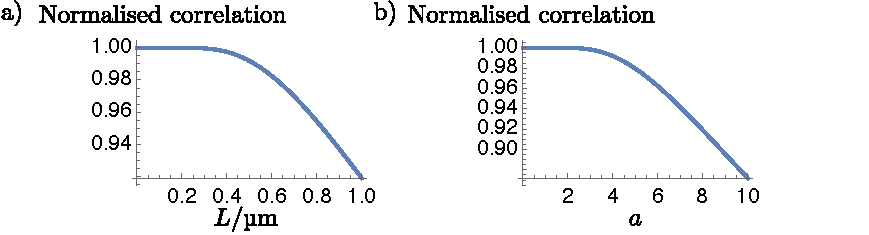
\includegraphics{./mathematica/correlation_analysis}
  \caption{}
  \label{fig:correlation_analysis}
\end{figure}

\subsection{Full width half maximum}

The correlation of two signals is not an absolute error which can be used to make predictions about real-world systems. So, the Full Width at Half Maximum of each of the two signals was considered as this property, in Gaussian-like functions, should provide an analogue for $\sigma(z)$ which may be compared absolutely.
\begin{align*}
\text{PSF}(x,...) &- \lim_{x\to0} \frac{\text{PSF}(x,...)}{2} = 0 \\
\implies \text{FWHM}_{\text{Expected}} &= 2x \\
&= \left|-\frac{\sqrt{2} c \sqrt{\ln{2} +2 i \pi  n} (a L+L_{\text{end}})}{L_{\text{end}}}\right|,n\in \mathbb{Z}
%\text{FWHM}_{\text{Expected}} &= \frac{2 \sqrt{3}}{\sqrt{\frac{a^2 L^2}{c^2 (a L+L_{\text{end}})^2}+\frac{3 L_{\text{end}}^2}{c^2 (a L+L_{\text{end}})^2}+\frac{3 a L_{\text{end}} L}{c^2 (a L+L_{\text{end}})^2}}}
\end{align*}
\begin{align*}
\text{PSF}_{\text{Reality}}(x,...) - \lim_{x\to0} \frac{\text{PSF}_{\text{Reality}}(x,...)}{2} = 0 \\
\intertext{This equation does not solve for $x$ so a Maclaurin expansion was used:}
= -\frac{L_{\text{end}} x^2}{4 \left(c^2 (a L+L_{\text{end}})\right)}+\frac{x^4 \left(a^2 L_{\text{end}} L^2+3 a L_{\text{end}}^2 L+3 L_{\text{end}}^3\right)}{48 c^4 (a L+L_{\text{end}})^3}+O\left(x^5\right)
\end{align*}
\begin{align*}
\implies \text{FWHM}_{\text{Reality}} &= \frac{2 \sqrt{3}}{\sqrt{\frac{a^2 L^2}{c^2 (a L+L_{\text{end}})^2}+\frac{3 L_{\text{end}}^2}{c^2 (a L+L_{\text{end}})^2}+\frac{3 a L_{\text{end}} L}{c^2 (a L+L_{\text{end}})^2}}}\\
\text{FWHM}_\text{Error} &= 2\frac{\text{PSF}_{\text{Expected}} - \text{PSF}_{\text{Reality}}}{\text{PSF}_{\text{Expected}} + \text{PSF}_{\text{Reality}}}\\
& = 2\frac{\sqrt{\ln{2}} \sqrt{a^2 L^2+3 a L_{\text{end}} L+3 L_{\text{end}}^2}-\sqrt{3} L_{\text{end}}}{\sqrt{\ln{2}} \sqrt{a^2 L^2+3 a L_{\text{end}} L+3 L_{\text{end}}^2}+\sqrt{3} L_{\text{end}}}
\end{align*}

When $L\to0$ this result of $\text{FWHM}_\text{Error}$ can be below zero, which would suggest that the result is not an accurate measure of the true error.
This is likely due to the process requiring a series expansion, at $x=0$; as the series expansion is only an approximation of the target function.
Since attaining error from the FWHM fails for small values of $L$ an analysis using area was considered.

\section{Magnetic tweezer alternate proof}\label{appendix:tweezertheory}

%The parameters from \eqref{eq:modelfitting} need to be reviewed and amended if one intends to link them to experimental data as one applies a known force and looks at the displacement of the bead from its initial position and not to stress and strain.

A bead moving through a viscous fluid can be described by Stokes' law \(F = 6 \pi \eta' r \nu \), where \(r\) is the radius of the bead and \(\nu \) is the critical velocity of the bead.
Stokes' law may be written as:

\begin{align}
 F &= 6 \pi \eta' r \frac{dx}{dt} \\
 \implies \frac{F}{\pi r^2} &= 6 \eta' \frac{d}{dt}\frac{x}{r} \\
 \implies \sigma &= 6 \eta' \frac{\epsilon}{dt}
 \intertext{Giving the equation of a dash-pot}
 \dot{\epsilon} = \frac{\sigma}{\eta}
\end{align}

To model the elastic spring, the elastic response of the tissue due to the bead displacement is approximated by the Thomson's solution of a point force in an infinite isotropic medium~\cite{l.d.landaue.m.lifshitzTheoryElasticity1970}.
The displacement (\(\mathbf{u}\)) in cylindrical coordinates (\((p,z)\)) for a point force (\(F_z\)) located at the origin and directed along the (\(z\)) axis is given by:

\begin{align}
 \mathbf{u} = \frac{F_z}{4 \pi \mu r }\left[ \frac{pz}{4(1-v)r^2} \mathbf{\hat{p}}+\left(1- \frac{p^2}{4(1-v)r^2}\right)\mathbf{\hat{z}}\right]\label{eq:thomsons}
\end{align}

Where \(\mathbf{\hat{p}}\) and \(\mathbf{\hat{z}}\) are unit vectors, \(\mu \) is the shear modulus (deformation at constant volume) and \(\nu \) is Poisson's ratio (a negative ratio of transverse to axial strain of a specimen, under an axial force).
As only forces in the \(\mathbf{\hat{z}}\) direction are being considering, Equation~\eqref{eq:thomsons} becomes:

\begin{align}
 u_z &= \frac{F_z}{4 \pi \mu r }\left[\left(1- \frac{p^2}{4(1-v)r^2}\right)\right]
 \intertext{Evaluating the displacement only on the \(z\) axis where \(p=0\), reduces this to:}
 \nabla z &= \frac{F_z}{4\pi \mu r}
 \intertext{In the close proximity to the bead of radius \(r_{\text{bead}} \), the displacement is given by:}
 \frac{\nabla z}{r_{\text{bead}}} = \frac{1}{4 \mu} \frac{F_z}{\pi r_{\text{bead}}^2} & \implies \epsilon = \frac{1}{4\mu} \sigma
\end{align}
Which is equivalent to~\eqref{eq:linearspring} when substituting \(E \) with \(4\mu \).
